\documentclass[12pt]{article}

\usepackage[utf8]{inputenc}
\usepackage[T1]{fontenc}
\usepackage[polish,provide=*]{babel}
\usepackage{lmodern}
\usepackage{amsmath}
\usepackage{latexsym,amsfonts,amssymb,amsthm,amsmath}
\usepackage{enumitem}
\usepackage{hyperref}
\usepackage{float}
\usepackage{graphicx}
\usepackage{subcaption}
\usepackage{booktabs}
\graphicspath{{./images/}}

\setlength{\parindent}{0in}
\setlength{\oddsidemargin}{0in}
\setlength{\textwidth}{6.5in}
\setlength{\textheight}{8.8in}
\setlength{\topmargin}{0in}
\setlength{\headheight}{18pt}

\title{Pomiar Zawartości Radonu w Powietrzu}
\author{Kacper Kłos}

\begin{document}

\maketitle

Abstract

\newpage
\section{Wstęp}
W owym raporcie przedstawimy wyniki jakie uzystakliśmy przy badaniu zawartości radonu w powietrzu obecnym w różnych pomieszczeniach. Do tego spróbójemy wyznaczyć zależność odbieranego promieniowania w funkcji odległości źródła od detektora promieniowania.

\section{Podstawy Teoretyczne}
Jedyne prawo fizyczne z którego będziemy korzystać jest prawo rozpadu, mówiące że ilość rozpadów promieniotwórczych jest wprost proporcjonalna do ilości rozpadanego izotopu.
\[
	\frac{dN(t)}{dt} = - \lambda N
\]
Gdzie lambda jest dodatnią stałą zależną od izotopu, a znak minus oznacza że ilość jąder maleje z czasem. Rozwiązując to równanie dochodzimy do zależności:
\begin{equation}
	N(t) = N(0) e^{-\lambda t}
	\label{eq:decay}
\end{equation}


\section{Układ Doświadczalny}

W pomiarach zależności od promieniowania od odległości jak i wyznaczania zawartości radonu w powietrzu skorzystamy z detektora promieniowania (dokładna budowa opisana w \cite{skrypt}) który wyznacza ilość zarejestrowanych rozpadów w danym przedziale czasowym.

Układ jaki wykorzystamy do zmierzenia zależności zmierzonego promieniowania od odległości widnieje na rys. \ref{fig:diagram}.
\begin{figure}[H]
	\centering
	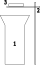
\includegraphics[scale=1]{układ}
	\label{fig:diagram}
	\caption{Układ pomiarowy wykorzystywany w doświadczeniu. 1 - miernik promieniowania, 2 - stojak z linijką, 3 - promieniotwórczy materiał.}
\end{figure}

Do zmierzenia zawartości radonu w powietrzu wykorzystamy pomiar polonu będący efektem rozpadu radonu. Aby wyznaczyć ilość polonu w powietrzu wykorzystamy metodę opisaną przez Markova \cite{equation}. Dzielimy pomiar na 3 fazy z przerwami:
\begin{enumerate}
	\item 5 min - pompowanie powietrza na filtr
	\item 1 min - przerwa
	\item 3 min - mierzenie promieniowania generowanego przez filtr
	\item 3 min - przerwa
	\item 3 min - mierzenie promieniowania generowanego przez filtr
\end{enumerate}
Graficznie widoczny na rys.
\begin{figure}[H]
	\centering
	\includegraphics[scale=0.7]{cycle}
	\label{fig:cycle}
	\caption{Graficzna reprezentacja cyklu (źródło:~\cite{skrypt})}
\end{figure}
Do pompowania wykorzystamy odkurzacz z podłączonym miernikiem objętości gazu.
Stosując wzór \eqref{eq:decay} wraz z danymi pochodzącymi z \cite{skrypt} otrzymamy wzór:
\[
	C_A = \frac{7{,}3 \times 10^{-5} (N_1 - N_2)}{\epsilon \, \nu \, \eta}
\]
We wzorze $N_i$ oznacza pomiar zarejestrowanych rozpadów w pierwszymi i drugim okresie, $\epsilon$ to wydajność miernika w rejestrowaniu cząstek, $\eta$ jest efektywnością zatrzymywanie produktów rozpadu na filtrze oraz $\nu$ to prędkość pompowania objęctości powietrza.

W dalszej części przyjmiemy że $\eta \approx 1$ jako że prawdziwa wartość jest tak bliska $1$ że nie będziemy w stanie jej dokładnie wyznaczyć. Także założymy $\epsilon \approx 0{,}0875$, jako że próbkę stawiamy na detektor połowa z cząstek poleciała w przeciwnym kierunku, a także zakładamy że $17{,}5\%$ cząstek które poleciały w stronę detektora do niego nie dotarły i zostały wykryte. Nasze oszacowanie opieramy na pracy \cite{scynt} w której efektywność scyntylatora jest wspomniana jako $33--44\%$, prze założeniu że nasz scyntylator jest raczej jednym z tych mniej dokładnych użyjemy wartości $35\%$. Następną składową jest to że nie wszystkie cząstki alpha dolecą do urządzenia przez ich silną interakcje z materią, pozyskując się \cite{alpha_range} zakładamy że $45\%$ cząstek nie doleci do detektora. Mnożąc te dwie wartości otrzymujemy wcześniej wspomniane $17{,}5$ oraz biorąc pod uwagę geometrię $\epsilon \approx 0{,}0875$. Zatem w analizie danych będziemy stosować wzór:

\begin{equation}
	C_A = \frac{83{,}43 \times 10^{-5} (N_1 - N_2)}{\nu}
	\label{eq:markov}
\end{equation}

\section{Wyniki Pomierów}
Wpierw ustawiamy próbkę radioaktywnego Th na stojaku (rys. \ref{fig:diagram}) w takiej pozycji mierzymy zarejestrowane rozpady w ciągu $t=120s$ i przedstawiamy w tab. \ref{tab:distance_measurments}.
\begin{table}[H]
	\centering
	\begin{tabular}{c|c|c}
		\toprule
		Nr & $N$ [Bq] & $d$ [cm] \\
		\midrule
		1  & 36       & 1        \\
		2  & 22       & 2        \\
		3  & 12       & 3        \\
		4  & 10       & 4        \\
		5  & 6        & 5        \\
		\bottomrule
	\end{tabular}
	\caption{Pomiary natężenia promieniowania $N$ w funkcji odległości źródła od góry detektora $d$.}
	\label{tab:distance_measurments}
\end{table}
Jako błąd zarejestrowanych pomiarów przyjmiemy $u(N) = \sqrt{N}$ a błąd dystansu uznamy za połowę podziałki $u(d) = 0.05 cm$.
Dla lepszego zrozumienia danych możemy przedstawić je na wykresie~\ref{fig:distance}.

\begin{figure}[H]
	\centering
	\includegraphics[scale=0.7]{distance}
	\label{fig:distance}
	\caption{Zależność zarejestrowanych rozpadów $N$ od odległości próbki od detektora $d$}
\end{figure}

Zależność na wykresie~\ref{fig:distance} możemy zbadać dokładniej dopasowując prostą do wykresu log-log.
\begin{figure}[H]
	\centering
	\includegraphics[scale=0.7]{distance_log}
	\label{fig:distance_log}
	\caption{Zależność logarytmu z zarejestrowanych rozpadów $N$ od logarytmu odległości próbki od detektora $d$}
\end{figure}
Otrzymane przez nas dopasowanie posiada parametry:
\[
	a = -1{,}0 \pm 0{,}1, \quad b = 3{,}6 \pm 0{,}1
\]
Oznacza to że $N \propto \frac{1}{d}$.


Następnie wykonując cykl Markova (rys.~\ref{fig:cycle}) będziemy badać stężenie polonu w powietrzu różnych środowisk. Wpierw badamy powietrze nad stertą kamieni wydobytych pewien czas temu, potem korytarza przed pokojem w którym wykonujemy doświadczenie i na koniec na dworze przez okno pokoju.
\begin{table}[H]
    \centering
    \begin{tabular}{c|cc|cc}
        \toprule
        Środowisko & $N_1$ [Bq] & $N_2$ [Bq] & $V_{\text{przed}}$ [m$^3$] & $V_{\text{po}}$ [m$^3$] \\
        \midrule
        Kamienie & 132 & 95  & 2479{,}45 & 2483{,}13 \\
        korytarz & 49  & 35  & 2483{,}13 & 2486{,}95 \\
        podwórze & 91  & 76  & 2486{,}95 & 2490{,}87 \\
        \bottomrule
    \end{tabular}
    \caption{Pomiar rozpadów $N_i$ w pierwszym i drugim cyklu (rys.~\ref{fig:cycle}) oraz objętości zmierzone przed oraz po fazie pompowania}
    \label{tab:density_measurments}
\end{table}
Za błąd pomiarowy rozpadów ponownie uznamy $u(N_i) = \sqrt{N_i}$ a błąd z jakim odczytujemy objętość to $u(V_i) = 0{,}01 \text{m}^3$ oraz czasu pompowania $u(t_p) = 1s$ uznajemy za marginalnie mały w porównaniu z błędem jaki będzie pochodzić od rozpadów.
Ze wzoru na propagację błędu otrzmamy że błąd wzoru \eqref{eq:markov} wynosi:

\[
	u(C_A) = \frac{83{,}43 \times 10^{-5} \sqrt{N_1 + N_2}}{\nu}
\]

Tak wyznaczone wartości ze wzoru \eqref{eq:markov} oraz z błędu powyżej wypisujemy w tab. \ref{tab:concentration_results}.

\begin{table}[H]
    \centering
    \begin{tabular}{c|cc}
        \toprule
        Środowisko & $C_A$ [Bq~m$^{-3}$] & $u(C_A)$ [Bq~m$^{-3}$] \\ 
        \midrule
        Kamienie & 25 & 11 \\
        korytarz & 9  & 6 \\
        podwórze & 10  & 9 \\
        \bottomrule
    \end{tabular}
    \caption{Pomiar rozpadów $N_i$ w pierwszym i drugim cyklu (rys.~\ref{fig:cycle}) oraz objętości zmierzone przed oraz po fazie pompowania}
    \label{tab:concentration_results}
\end{table}

\section{Podsumowanie}
W powyższym raporcie udało nam się wyznaczyć zależność odbieranych cząstek alfa od odległości. Wyznaczona przez dopasowanie liniowe do wzoru $\log(N) = a \log(r) + B$ daje nam wartości $a = -1{,}0 \pm 0{,}1$ oraz $b = 3{,}6 \pm 0{,}1$, które mówią nam o zależności $N \propto \frac{1}{r}$.
Następnie badaliśmy obecność Po-$218$ w powietrzu, w celu ustalenia zawartości Rn-$222$ który rozpada się na wspomniany polon. Badanie przeprowadziliśmy przy pomocy wzoru wyprowadzonego przez Markova \cite{equation}, badaliśmy trzy różnych otoczenia i otrzymaliśmy wartości: $C_{A_s} = 25 \pm 11$ [Bq~m$^{-3}$] dla sterty kamieni,
$C_{A_c} = 9 \pm 6$ [Bq~m$^{-3}$] dla korytarza budynku w którym było wykonywane doświadczenia oraz $C_{A_o} = 10 \pm 9$ [Bq~m$^{-3}$] w przypadku podwórza.

Możemy zastanowić się jakich wartości spodziewalibyśmy się w powyższych eksperymentach. Wiemy że promieniowanie wraz z odległością powinno być pewnego rodzaju kompozycją odwrotności kwadrata (ponieważ cząstki rozchodzą się po sferze), a także spadku wykładniczego wywołanego coraz mniejszą ilością cząstek dochodzących do detektora. Otrzymane przez nas dopasowanie nie przedstawia takiego stanu rzeczy, lecz z powodu ogromnych błędów pomiarowych, równie dobrze może się tak zachowywać ale pomiar nie był na tyle dokładny by to zaobserwować. Posłógując się raportem \cite{concentration} możemy określić jakość naszych pomiarów zawartości radonu w powietrzu. Widzimy że różnica jest duża, niemniej jednak udało nam się uchwycić pewne niuanse, powietrze nad kamieniami ma zauważalnie większą obecność radonu co zgadza się z badaniem w którym powietrze bliżej centrum ziemi ma większą koncentrację tego pierwiastka.

Różnice między otrzymanymi wartościami a otrzymanymi w innych publikacjach pochodzi z ogromnego błędu obecnego w naszych pomiarach. Błąd statystyczny pomiaru zarejestrowanych cząstek już posiada ogromny błąd $\sqrt{N}$, w dodatku w ocenie obecności radonu użyliśmy bardzo ogólnych oszacowań dotyczących wydajności rejestracji cząstek, oraz założyliśmy że wszystkie cząstki zatrzymują się na filtrze podczas pompowania. Wszystkie te czynniki sprawiają że nasz pomiar jest obarczony dużymi błędami.

\newpage

\begin{thebibliography}{5}

	\bibitem{skrypt}
	\emph{Pomiar Zawartości Radonu w Powietrzu}, Uniwersytet Warszawski.
	\bibitem{equation}
	\emph{Atomnaja Energia 12}, K.P. Markov, N.W. Rijabov, K.N. Stas.
    \bibitem{scynt}
    \url{https://scintacor.com/wp-content/uploads/2021/09/Comparisons-of-new-simple-methods-in-fabricating-ZnS-Ag-scintillatiors-for-detecting-alpha-particles.pdf}, \emph{Comparison of New Simple Methods in Fabricating ZnS(Ag) Scintillators for Detecting Alpha Particles}, Seung Kyu LEE, Shin Yang KANG, Doh Yun JANG, Cheol Ho LEE, Sang Mook KANG, Byoung Hwi KANG, Woo Gyo LEE, and Yong Kyun KIM. 
    \bibitem{alpha_range}
    \url{https://www.rad-proceedings.org/papers/RadProc.2018.25.pdf}, \emph{ALPHA SELF-ABSORPTION EVALUATION IN RADIOMETRIC FILTER MATERIAL FOR THE NATURAL RANGE OF ALPHA ENERGY (5-9 MeV)}, M. Y.A. Mostafa, M.V. Zhukovsky.
    \bibitem{concentration}
    \emph{Promieniotwórczość a życie: problem ryzyka związanego z promieniowaniem jonizującym, Raport Nr 12, Dział Szkolenia IPJ}, L. Dobrzyński i E. Droste, Warszawa 1999


\end{thebibliography}

\end{document}
